\documentclass{article}
\usepackage{amsmath}
\usepackage{amsthm}
\usepackage{amsfonts}
\usepackage{bm}
\usepackage[usenames,dvipsnames]{xcolor}
\usepackage{tikz}
\usepackage{hyperref}

\hypersetup{
    colorlinks,
    linkcolor={red!30!black},
    citecolor={blue!50!black},
    urlcolor={blue!80!black}
}


\begin{document}

\title{Method of Characteristics}
\author{ \vspace{-10ex} }
\date{ \vspace{-10ex} }
\maketitle

\tableofcontents

\section{Introduction}

The method of characteristics
is a method of solving partial differential equations (PDE).
%
We'll distinguish two cases.
\begin{enumerate}
\item Semi-linear:
  $$a(x, y) \, u_x + b(x, y) \, u_y = f(x, y, u).$$
  If $f(x, y, u) = f_1(x, y) - c(x, y) \, u$,
  then this becomes a linear PDE.

\item Quasi-linear:
  $$a(x, y, u) \, u_x + b(x, y, u) \, u_y = f(x, y, u).$$
  The difference is that the coefficients $a$ and $b$
  are now also functions of $u$.
\end{enumerate}
The method work pretty much in the same way
for the two cases.
The difference is mainly the mathematical difficulty.


\section{Semi-linear Cauchy problem}

\subsection{Cauchy problem}

If a differential equation
\begin{equation}
a(x, y) \, u_x  + b(x, y) \, u_y = f(x,y, u),
\label{eq:PDE_semilinear}
\end{equation}
is coupled with the initial condition (think of $y$ at time $t$)
\begin{equation}
u(x, 0) = u_0(x).
\label{eq:initialcondition}
\end{equation}
The pair \eqref{eq:PDE_semilinear} and \eqref{eq:initialcondition}
is call a semi-linear Cauchy problem.


\subsection{Solution is a 3D surface}

The solution of the Cauchy problem is a surface\footnote{
The $u(x, y)$ on the right-hand side denotes a function,
the $u$ on the left-hand side is the $z$ coordinate.
}
$$
u = u(x, y)
$$
in the 3D ($x$-$y$-$u$) space.
Why? Because \eqref{eq:PDE_semilinear}
can be thought as an equation specifying the time evolution
(we call $y$ time)
of the single-variable function $u_y(x) \equiv u(x, y)$ of $x$.
At $y = 0$, the function corresponds to a curve in the $x$-$u$ plane:
$u(x, 0) = u_0(x)$ by \eqref{eq:initialcondition}
(Figure \ref{fig:solsurface}).
%
At a later $y$, we advance the curve along $y$
according to
$$
\frac{\partial u} {\partial y}
= \frac{ f(x, y, u) - a(x, y) u_x} { b(x, y) }.
$$
That is, we integrate it by
$u(x, y+\Delta y) = u(x, y) + (\partial u/\partial y) \, \Delta y$.
Keep doing this yields $u_y(x)$ for any $y$.

\begin{figure}[h]
\centering
  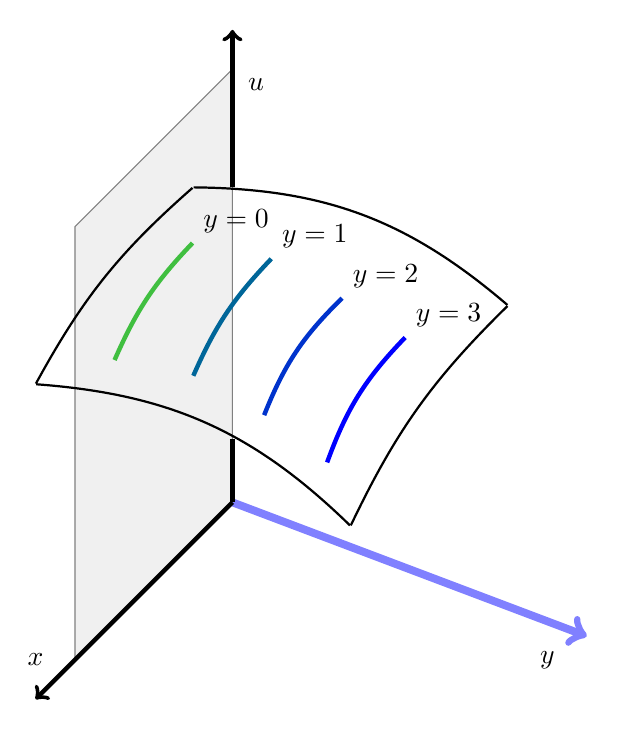
\begin{tikzpicture}
  [enode/.style={minimum size=0, inner sep=0}]

  % u-x plane
  \draw[thin, fill=gray!12!white, draw=gray]
    (2.5, -1.5) -- (0.5, -3.5) -- (0.5, 2) -- (2.5, 4) -- cycle;

  % y axis
  \draw[ultra thick, ->, draw=blue!50!white,line width=1mm] (2.5, -1.5) -- (7, -3.2);
  \node[enode] (y) at (6.5, -3.5) {$y$};

  % u axis (vertical)
  \draw[ultra thick, ->, draw=black] (2.5, 2.5) -- (2.5, 4.5);
  \draw[ultra thick, draw=black] (2.5, -1.5) -- (2.5, -0.7);
  \node[enode] (u) at (2.8, 3.8) {$u$};

  % x axis
  \draw[ultra thick, ->, draw=black] (2.5, -1.5) -- (0.0, -4.0);

  \node[enode] (x) at (0, -3.5) {$x$};
  \node[enode] (x1) at (0, 0) {};
  \node[enode] (x2) at (4, -1.8) {} edge [thick, bend right=20] (x1);
  \node[enode] (x3) at (6, 1.0) {} edge [thick, bend right=10] (x2);
  \node[enode] (x4) at (2, 2.5) {} edge [thick, bend right=10] (x1)
                                   edge [thick, bend left=20] (x3);

  \node[enode] (x1a) at (1.0, 0.3) {};
  \node[enode, label={10:$y=0$}] (x4a) at (2.0, 1.8) {}
         edge [bend right=10, ultra thick, draw=green!50!gray] (x1a);

  \node[enode] (x1b) at (2.0, 0.1) {};
  \node[enode, label={10:$y=1$}] (x4b) at (3.0, 1.6) {}
         edge [bend right=10, ultra thick, draw=blue!60!green] (x1b);

  \node[enode] (x1c) at (2.9, -0.4) {};
  \node[enode, label={10:$y=2$}] (x4c) at (3.9, 1.1) {}
         edge [bend right=12, ultra thick, draw=blue!80!green] (x1c);

  \node[enode] (x1d) at (3.7, -1.0) {};
  \node[enode, label={10:$y=3$}] (x4d) at (4.7, 0.6) {}
         edge [bend right=12, ultra thick, draw=blue] (x1d);

  \end{tikzpicture}
  \caption{
    \label{fig:solsurface}
    At $y = 0$, the initial condition specifies a 3D curve (green)
    $u(x, 0) = u_0(x)$ in the $x$-$u$ plane.
    As $y$ increases, the curve progresses along the $y$ axis,
    and updates itself according to the PDE:
    $\partial u/\partial y = (f - a u_x)/b$.
    The entire history of the evolved curves at different $y$
    forms a 3D surface.
    Thus, the solution of the Cauchy problem is a surface $u = u(x,y)$.
  }
\end{figure}


Thus, by solving the PDE,
we effectively develop the curve $(x, 0, u_0(x))$
from the initial condition
to a surface $(x, y, u(x, y))$
(Figure \ref{fig:solsurface}).
%
This surface of the Cauchy problem
is referred to the \emph{integral surface} below.


\subsection{Geometric characterization}

Let us rewrite the desired solution as
$$
F(x, y, u) = u(x, y) - u = 0.
$$
which is an equation of a 3D surface.\footnote{
This is different way of writing a surface.
%
This expression in terms of $F$
treats $x$, $y$ and $u$ on equal footing.
For example,
$F(x, y, u) = x^2 + y^2 +u^2 - 1$
is the surface of unit sphere.
The normal is $(F_x, F_y, F_u)$
along which $F$ increases fastest.
%
By solving $F=0$ for $u$,
we recover the form majorized for $u$, e.g.,
$
u = \sqrt{1 - x^2 - y^2}.
$
}
%
Here, $u(x, y)$ is a function of $x$ and $y$,
whereas the second ``$u$'' is the argument
of function $F(x, y, u)$.

Now \eqref{eq:PDE_semilinear} can be written as
a dot product
$$
(a, b, f) \cdot (u_x, u_y, -1) = 0.
$$
or
\begin{equation}
(a, b, f) \cdot (F_x, F_y, F_u) = 0.
\label{eq:dotproduct1}
\end{equation}

\begin{figure}[h]
  \centering
  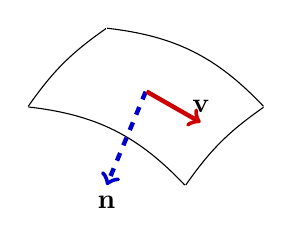
\begin{tikzpicture}
  [enode/.style={minimum size=0, inner sep=0}]
  \node[enode] (x1) at (0, 0) {};
  \node[enode] (x2) at (2, -1) {} edge [bend right=20] (x1);
  \node[enode] (x3) at (3, 0) {} edge [bend right=10] (x2);
  \node[enode] (x4) at (1, 1) {} edge [bend right=10] (x1) edge [bend left=20] (x3);

  \node[enode, label={-90:$\mathbf n$}] (n) at (1, -1) {};
  \node[enode, label={90:$\mathbf v$}] (v) at (2.2, -0.2) {};
  \node[enode] (x) at (1.5, 0.2) {}
        edge [ultra thick, dashed, ->, draw=blue!80!black] (n)
        edge [ultra thick, ->, draw=red!80!black] (v);
  \end{tikzpicture}
  \caption{
    \label{fig:characteristic_direction}
    The vector $\mathbf v = (a, b, f)$ gives
    a direction perpendicular to the normal $\mathbf n$
    of the surface.
    %
    Thus, $\mathbf v$ always lies on the surface of the solution.
  }
\end{figure}


The vector $\mathbf n = (F_x, F_y, F_u) = (u_x, u_y, -1)$
is the normal of the surface $F$.
So \eqref{eq:dotproduct1}
means that the vector $\mathbf v = (a(x, y), b(x, y), f(u, x, y))$
is perpendicular to the normal,
and thus lies on the tangent plane of the surface
(Figure \ref{fig:characteristic_direction}.



\subsection{Characteristic curve}

So if we start from a point of the initial curve
(which lies on the integral surface)
and move along the direction of $\mathbf v$,
the trajectory always lies on the integral surface.
%
This curve is called the \emph{characteristic curve}.

Now a 3D curve can be parameterized by a real number $t$
$$
\mathbf p(t) = (x(t), y(t), u(t)).
$$
So its derivative, or the tangent vector, is
$$
\mathbf p'(t) = (x'(t), y'(t), u'(t))^T.
$$
This vector must be parallel to $\mathbf v$,
since they both represent the tangent direction of the characteristic curve.
Thus,
$$
\frac{ dx(t)/dt } { a(x, y) }
=
\frac{ dy(t)/dt } { b(x, y) }
=
\frac{ du(t)/dt } { f(x, y, u) }.
$$
Written in a more compact differential form
\begin{equation}
\frac{ dx } { a(x, y) }
=
\frac{ dy } { b(x, y) }
=
\frac{ du } { f(x, y, u) }.
\label{eq:characteristic_curve_diff}
\end{equation}

This is the most important equation
of the method of characteristics.


\subsection{Curve and surface}

A common question is the following.
A characteristic curve is by definition a curve,
and that is what we will get by solving
\eqref{eq:characteristic_curve_diff}.
%
So how does it help us to find the integral surface
for the solution of the Cauchy problem?

The answer is that the solution to
\eqref{eq:characteristic_curve_diff}
yields a \emph{family} of characteristic curves,
distinguished by some free parameters
given in terms of the constants of integration.
%
We can use these constants of integration
to specify where the characteristic curve starts
at $y = 0$ (in terms of the coordinates on $x$-$u$ plane).
%
So if the initial condition is a single point
in the $x$-$u$ plane,
there is indeed only one characteristic curve
(red in Figure \ref{fig:characteristic_curve}).
%
But in our case, the initial condition is another curve
(green in Figure \ref{fig:characteristic_curve}),
specified by $u(x, 0) = u_0(x)$.
%
So each point on the initial curve will develop a characteristic curve
as $y$ increases.
%
These characteristic curves will spread and cover
the entire integral surface
corresponding to the solution of the Cauchy problem.

\begin{figure}[h]
  \centering
  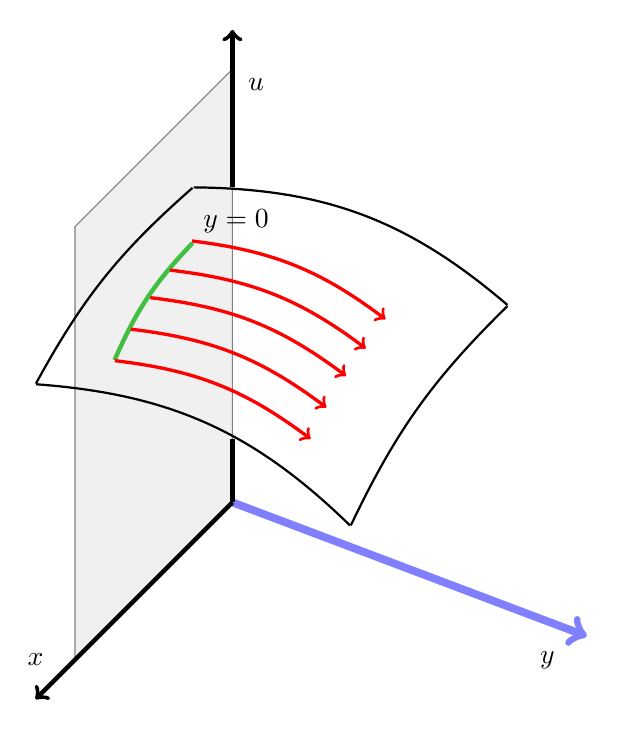
\begin{tikzpicture}
  [enode/.style={minimum size=0, inner sep=0}]

  % u-x plane
  \draw[thin, fill=gray!12!white, draw=gray]
    (2.5, -1.5) -- (0.5, -3.5) -- (0.5, 2) -- (2.5, 4) -- cycle;

  % y axis
  \draw[ultra thick, ->, draw=blue!50!white,line width=1mm] (2.5, -1.5) -- (7, -3.2);
  \node[enode] (y) at (6.5, -3.5) {$y$};

  % u axis (vertical)
  \draw[ultra thick, ->, draw=black] (2.5, 2.5) -- (2.5, 4.5);
  \draw[ultra thick, draw=black] (2.5, -1.5) -- (2.5, -0.7);
  \node[enode] (u) at (2.8, 3.8) {$u$};

  % x axis
  \draw[ultra thick, ->, draw=black] (2.5, -1.5) -- (0.0, -4.0);

  \node[enode] (x) at (0, -3.5) {$x$};
  \node[enode] (x1) at (0, 0) {};
  \node[enode] (x2) at (4, -1.8) {} edge [thick, bend right=20] (x1);
  \node[enode] (x3) at (6, 1.0) {} edge [thick, bend right=10] (x2);
  \node[enode] (x4) at (2, 2.5) {} edge [thick, bend right=10] (x1)
                                   edge [thick, bend left=20] (x3);

  \node[enode] (s1) at (1.0, 0.3) {};
  \node[enode, label={10:$y=0$}] (s4) at (2.0, 1.8) {}
        edge [bend right=10, ultra thick, draw=green!50!gray] (s1);

  \node[enode] (t1) at (3.5, -0.7) {}
        edge [bend right=15, very thick, draw=red, <-] (s1);

  \node[enode] (s2) at (1.2,  0.7) {};
  \node[enode] (t2) at (3.7, -0.3) {}
        edge [bend right=15, very thick, draw=red, <-] (s2);

  \node[enode] (s3) at (1.45,  1.1) {};
  \node[enode] (t3) at (3.95,  0.1) {}
        edge [bend right=15, very thick, draw=red, <-] (s3);

  \node[enode] (s4) at (1.70,  1.45) {};
  \node[enode] (t4) at (4.20,  0.45) {}
        edge [bend right=15, very thick, draw=red, <-] (s4);

  \node[enode] (s5) at (1.98,  1.82) {};
  \node[enode] (t5) at (4.45,  0.82) {}
        edge [bend right=15, very thick, draw=red, <-] (s5);

  \end{tikzpicture}
  \caption{
    \label{fig:characteristic_curve}
    Each point on the curve specified by the initial condition (green)
    can develop a characteristic curve (red).
    The total of the characterstic curves is
    the desired integral surface.
  }
\end{figure}







\subsection{Decomposition into ODEs}

Now \eqref{eq:characteristic_curve_diff}
can be decoupled to a pair of equations
(any two of the three pairings will do)
$$
\begin{aligned}
\frac{dx}{dy} &= \frac{ a(x, y) } { b(x, y) }, \\
\frac{du}{dy} &= \frac{ f(x, y, u) } { b(x, y) }.
\end{aligned}
$$

Then by combining the solutions of the above two
ordinary differential equations (ODEs),
we can get a solution to the full PDE.
%
We will show how this is actually done through an example.
%
We shall see that the ``combination'' of the two ODEs involves establishing
a relationship between the two constants of the integration.




\subsection{Example 1.}

Problem.
For constant $a$, $b$ and $f$, solve
$$
a u_x + b u_y = f
\qquad
u(x, 0) = \sin(x).
$$

So \eqref{eq:characteristic_curve_diff} reads
$$
\frac{ dx } { a } =
\frac{ dy } { b } =
\frac{ du } { f }.
$$
Then we decompose this to a pair of equations
$$
\begin{aligned}
\frac{ dx } { a } &= \frac{ dy } { b }, \\
\frac{ dy } { b } &= \frac{ du } { f }.
\end{aligned}
$$
From the first equation, we get
$x = (a/b) y + C_1$;
from the second, we get
$u = (f/b) y + C_2$.


\subsection{Relation between the constants of integration}


We now show that there is a functional relationship
between the two constants $C_1$ and $C_2$.
%
First recall that,
any given point on the initial curve
$(x_0, y_0, u_0) = (x_0, 0, u_0(x_0))$
starts a distinct characteristic curve
as $y$ increases.
%
Since the number $x_0$ is the single parameter
that specifies the starting point,
it will also be the only parameter
specifying the characteristic curve.
%
This means that $C_1$ must be a function
of $x_0$, and $C_2$ another function of $x_0$:
$$
\begin{aligned}
C_1 &= g_1(x_0), \\
C_2 &= g_2(x_0).
\end{aligned}
$$
By eliminating $x_0$,
we get a functional relationship between $C_1$ and $C_2$:
%
\begin{equation}
C_2 = G(C_1),
\label{eq:C1C2_relationship}
\end{equation}
where $G = g_2 \circ g_1^{-1}$.
%
In practice, we do not need $g_1$ and $g_2$,
and the function $G$ can be sought
directly from the initial condition,
as illustrated below.


\subsection{Example 1 continued}

Back to example 1, \eqref{eq:C1C2_relationship} means
\begin{equation}
u - \frac f b y = G\left(x - \frac a b y\right).
\label{eq:relation_example1}
\end{equation}
The functional form is determined from the initial condition:
at $y = 0$, $u = \sin(x)$.
So the function $G$ is determined as
$G(x) = u = \sin(x)$.
Using this in \eqref{eq:relation_example1}, we get
the full solution
$$
u - \frac f b y = \sin \left(x - \frac a b y\right).
$$


\subsection{Change-of-variables interpretation}


We now give a slightly different explanation
on the functional relationship between the constants
of integration.
%
A characteristic curve can be thought as
a geometric transformation (or, a map)
in the $x$-$u$ plane,
parameterized by $y$.
%
That is, given an input point $(x_0, u_0)$
at time $y = 0$,
the characteristic curve is a black box
that outputs the new coordinates $(x, u)$
at time $y$.
%
The inverted map will do the reverse:
given the coordinates $(x, u)$ at time $y$,
it outputs $(x_0, u_0)$ at time $0$
as some functions of $x$ and $u$.
%
In other words,
the transformation between $(x, u)$ and $(x_0, u_0)$
is merely a change of variables.
%
In the above example,
this geometric transformation is simply a linear shift
\begin{equation}
\begin{aligned}
x_0 &= x - \frac{a}{b} y, \\
u_0 &= u - \frac{f}{b} y.
\end{aligned}
\label{eq:geometric_transform}
\end{equation}
Now if the initial variables $x_0$ and $u_0$
satisfies some relationship, say $u_0 = G(x_0)$,
then the time-$y$ variables $x - (a/b) \, y$ and $u - (f/b) y$
must satisfy the same relationship.
%
This gives the full solution:
$$
u - \frac f b y = G\left( x - \frac a b y \right).
$$

In this case,
we identify $G(x)$
as the function given by the initial condition $u_0(x)$,
and the coordinates $x_0$ and $u_0$ on the initial curves
are just the two constants of integration $C_1$ and $C_2$.
%
Generally, the constants of integration $C_1$ and $C_2$
may have more involved expressions,
but their function remains the same:
to specify the initial point on the $x$-$u$ plane.
%
Since the initial condition specifies
a curve on the initial $x$-$u$ plane,
there must be a functional relationship
between $C_1$ and $C_2$.


\subsection{Generalization to more variables.}

The change-of-variables interpretation makes it
easy to generalize to a PDE with more variables.
%
Now consider the equation
$$
a_1 \, \frac{\partial u}{\partial x_1}
+
\cdots
+
a_n \, \frac{\partial u}{\partial x_n}
+
b \, \frac{\partial u}{\partial y}
=
f,
$$
where the coefficients $a_1, \dots, a_n, b$ and $f$
are functions of
$x_1, \dots, x_n, y$ and $u$.
%
The method of characteristics seeks the solution of
$$
\frac{dx_1}{ a_1 }
=
\cdots
=\frac{dx_n}{ a_n }
= \frac{dy}{ b }
= \frac{du}{ f }.
$$
Thus, we will get $n+1$ constants of integration
$C_1, \dots, C_n, C_{n+1}$
for $x_1, \dots, x_n, u$.
%
Again, these constants of integration
specify the position of the initial point
on the $(n+1)$-dimensional hyperplane at $y = 0$,
much like the Cartesian coordiantes
$x_{10}, \dots, x_{n0}, u_0$.

If the initial condition is a single equation,
$$
u(x_1, \dots, x_n, y = 0) = u_0(x_1, \dots, x_n).
$$
then the starting points spread over
a $n$-dimensional hypersurface.
%
Correspondingly,
we have only one relationship between the constants
of equations, say
$$
C_{n+1} = G(C_1, \dots, C_n).
$$
But if the initial condition is more detailed,
there are more restriction between the constants.
%
If there is only one initial point,
then all constants of integration are fixed.

\subsection{Example 2}

Problem.
For $x > 0$, solve
$$
x u_x + y u_y = x e^{-u}
\qquad
u(x, x^2) = x.
$$

Here, $a(x, y) = x$, $b(x, y) = y$, and $f(x, y, u) = x \, e^{-u}$.
So \eqref{eq:characteristic_curve_diff} reads
$$
\frac{ dx } { x } =
\frac{ dy } { y } =
\frac{ du } { x \, e^{-u} }.
$$
We form two equations
$$
\begin{aligned}
\frac{ dx } { x } &= \frac{ dy } { y}, \\
\frac{ dx } { x } &= \frac{ du } { x \, e^{-u} }.
\end{aligned}
$$
The solution of the first equation is
$d\ln x = d\ln y$ or
\begin{equation}
y = C_1 x.
\label{eq:example2_sol1}
\end{equation}
The second equation is
$dx = e^u \, du$ and the solution is
$e^u = x + C_2$.

Then we demand a functional relationship between $C_1$ and $C_2$ as before.
So $C_2 = G(C_1)$, or
$$
e^u - x = G(y/x).
$$
Using the initial condition with $y = x^2$ and $u = x$,
we determine the functional form of $G(x)$:
$$
G(x) = e^x - x.
$$
So the solution is
\begin{equation}
e^u - x = e^{y/x} - \frac{y}{x}.
\label{eq:example2_fullsol}
\end{equation}


\subsection{Another solution to Example 2}

Let us try to solve the same problem in a harder way.
We replace the pair by
$$
\begin{aligned}
\frac{ dx } { x } &= \frac{ dy } { y}, \\
\frac{ dy } { y } &= \frac{ du } { x \, e^{-u} }.
\end{aligned}
$$
The first equation still yields
\eqref{eq:example2_sol1}.
But the second equation becomes
$$
dy = \frac{y}{x} e^u du.
$$
This looks hard, but with the help of\eqref{eq:example2_sol1},
we get
$$
dy = C_1 e^u \, du,
$$
and $ y = C_1 \, e^u + C_2$.  So
$$
C_2 = y - C_1 e^u = y - \frac y x e^u.
$$
Again, we insist a functional relationship between $C_1$ and $C_2$:
$C_2 = G(C_1)$, and
$$
y - \frac y x e^u = G(y/x).
$$
Using the initial condition $u(x, x^2) = x$,
$$
G(x) = x^2 - x e^x,
$$
and
$$
y - \frac y x e^u = \left(\frac{y}{x}\right)^2  - \frac{y}{x} e^{y/x}.
$$
Multiplying both side by $-x/y$,
we get the same solution as \eqref{eq:example2_fullsol}.

The point of this exercise is to show that
sometimes, we have to first solve an easy equation,
then use the constant of integral obtained there
to simplify the other equation.


\section{Quasi-linear PDE}


We now turn to the quasi-linear case.
%
The difference from the semi-linear PDEs is
that in quasi-linear PDEs, $a$, $b$
are now functions of $u$.
%
The procedure is summarized below.

The characteristic curve is defined by
$$
\frac{ dx } { a(x, y, u) }
=
\frac{ dy } { b(x, y, u) }
=
\frac{ du } { f(x, y, u) }.
$$
Selecting two pairs and solving the corresponding ODEs,
we get two constants of integration.
$$
h(x, y, u) = C_1,
\qquad
j(x, y, u) = C_2.
$$
We then demand a functional relationship between $C_1$ and $C_2$: $C_2 = G(C_1)$.
Then
$$
j(x, y, u) = G(h(x, y, u)).
$$
The function $G$ will be found from the initial condition.


\subsection{Burger's equation}

Problem.
Solve Burger's equation from fluid mechanics,
$$
u \, u_x + u_y = 0,
\qquad
u(x, 0) = \phi(x).
$$

The characteristic equation is
$$
\frac{ dx } { u }
=
\frac{ dy } { 1 }
=
\frac{ du } { 0 }.
$$
The last equation simply means $u$ is a constant.
Thus we get our first constant of integral
$u = C_1$.

Now for the $x$-$y$ pair.
$$
dx = u \, dy = C_1 dy.
$$
Thus, we get the second constant of integration
$$
C_2 = x - C_1 y = x - u y,
$$

To combine the two, we
impose $C_1 = G(C_2)$, and
$$
u = G(x - u y).
$$
Using the initial condition, $y = 0$ and $u = \phi(x)$,
we get
$$
G(x) = \phi(x).
$$
So, the solution is given by the implicit form
$$
u = \phi(x - u \, y).
$$


\subsection{Example 3}

Problem.
Solve
$$
(y + u) u_x + y u_y = x - y.
$$

The characteristic curve is determined by
$$
\frac{ dx } { y + u }
=
\frac{ dy } { y }
=
\frac{ du } { x - y }.
$$

Using the fact
$$
\frac{a}{b} = \frac{c}{d}
\Longleftrightarrow
\frac{a + c}{b + d} = \frac{a}{b},
$$
for the $x$-$u$ pair, we have
$$
\frac{ dy } { y }
=
\frac{ d(x+u) } { (x + u) }
$$
The solution is $x+u = C_1 y$.

Similarly, for the $y$-$u$ pair, we get
$$
\frac{ dx } { y + u }
=
\frac{ d(y+u) } { x }.
$$
which gives
$(y+u)^2 - x^2 = C_2$.
%
Again, we demand a functional relationship between $C_1$ and $C_2$:
$C_2 = G(C_1)$.
So
\begin{equation}
(y+u)^2 - x^2 = G\left(\frac{x+u}{y}\right).
\label{eq:qs_ex3_sol1}
\end{equation}

\subsubsection*{Another pairing}

Note. We can also choose the $x$-$y$ pair, and
$$
\frac{ d(x - y) } { u }
=
\frac{ du } { x - y },
$$
which gives $(x - y)^2 - u^2 = C_3$.
So the functional relationship can also be
$$
(y+u)^2 - x^2 = G_1\left( (x-y)^2 - u^2 \right),
$$
or
\begin{equation}
(x-y)^2 - u^2 = G_2\left( \frac{x+u}{y} \right).
\label{eq:qs_ex3_sol2}
\end{equation}

Now \eqref{eq:qs_ex3_sol2} looks a bit different from \eqref{eq:qs_ex3_sol1},
do they represent the same solution?
The answer is yes.
Note
$$
\begin{aligned}
C_2 &= (y + u)^2 - x^2 =
\left(1 + \frac{u + x}{y}\right) \, (u - x + y) \, y
= \left(1 + C_1 \right) C_4, \\
C_3 &= (x - y)^2 - u^2 =
\left(1 - \frac{x + u}{y}\right) \, (u - x + y) \, y
= \left(1 - C_1\right) C_4,
\end{aligned}
$$
%
where $C_4 = (u - x + y) \, y$.
%
Thus, $C_2$ and $C_3$
represent different multiples of $C_4$.
%
Interestingly, the constant $C_4$ will show up directly
from the following alternative method.


\subsection{Example 3 solved more systematically}

The example can be solved more systematically.
Let us keep $dt$ and write,
$$
\begin{aligned}
\frac{dx}{dt} &= y + u \\
\frac{dy}{dt} &= y \\
\frac{du}{dt} &= x - y,
\end{aligned}
$$
This is a set of linear equations,
which can always be solved.
Namely,
$$
\frac{ d \mathbf v}{dt}
= \mathbf A \, \mathbf v
$$
can always be solved as $\mathbf v = \exp(t\mathbf A) \, \mathbf c$.

This is most readily done by linearly combining
equations to form eigenvectors,
for which the matrix $\mathbf A$ is diagonal.
$$
\begin{aligned}
\frac{dy}{dt} &= y \\
\frac{d(x + u)}{dt} &= x + u \\
\frac{d(u-x+y)}{dt} &= -(u-x+y),
\end{aligned}
$$
Thus,
$$
\begin{aligned}
y &= c_1 \, e^t, \\
x + u &=  c_2 \, e^t \\
u - x + y &= c_3 \, e^{-t},
\end{aligned}
$$
Now we can eliminate $t$, and
$$
\begin{aligned}
\frac{x + u}{y} &= \frac{c_2}{c_1} = C_1', \\
(u - x + y) \, y &= c_1 \, c_3 = C_2'.
\end{aligned}
$$
Here $C_1'$  and $C_2'$ are the two combined constants.
If we assume a functional relationship between them, then
$$
(u - x + y) \, y = G'\left( \frac{x+u}{y} \right).
$$

\subsection{Example 4}

Problem.
Solve
$$
x \, (y^2 + u) \, u_x - y \, (x^2 + u) \, u_y = (x^2 - y^2) \, u,
\qquad
u(x, 3x) = x^2.
$$

The characteristic equation is
$$
\frac{ dx } { x \, (y^2 + u) }
=
\frac{ dy } { -y \, (x^2 + u) }
=
\frac{ du } { (x^2 - y^2) \, u }.
$$
This is equivalent to
$$
\frac{ x \, dx } { x^2 \, (y^2 + u) }
=
\frac{ y \, dy } { -y^2 \, (x^2 + u) }
=
\frac{ du } { (x^2 - y^2) \, u }.
$$
Combining the $x$-$y$ pair, we get
$$
\frac{ d(\frac{x^2 + y^2}{2}) } { u \, (x^2 - y^2) }
=
\frac{ du } { (x^2 - y^2) \, u }.
$$
We get the first constant of integration
$C_1 = u - (x^2 + y^2)/2$.

Similarly we have
$$
\frac{ y \, dx } { x \, y \, (y^2 + u) }
=
\frac{ x \, dy } { -y \, x \, (x^2 + u) }
=
\frac{ du } { (x^2 - y^2) \, u }.
$$
After combining the $x$-$y$ pair, we get
$$
\frac{ d (x \, y) } { x \, y \, (y^2 - x^2) }
=
\frac{ du } { (x^2 - y^2) \, u }.
$$
This yields the second constant $x \, y \, u = C_2$.

We again impose the functional relationship, $C_2 = G(C_1)$,
$$
x \, y \, u = G(u - (x^2 +y^2)/2).
$$
Using the initial condition of $y = 3x, u = x^2$, we get
$$
3\, x^4 = G(-4 x^2),
$$
which means $G(y) = (3/16) y^2$.
$$
x y u = \frac{3}{16} \left( u - \frac{x^2+y^2}{2} \right)^2.
$$


\section{References}

YouTube tutorials
\begin{enumerate}
\item
Chris Tisdell, Method of characteristics, \url{https://www.youtube.com/watch?v=LpHqrlrU5pM}.
The principle of the method is described in this video.

\item
Chris Tisdell, How  to solve Burger's equation, \url{https://www.youtube.com/watch?v=5ZrwxQr6aV4}.
This and later videos are about quasi-linear PDEs.

\item
Chris Tisdell, How to solve quasi-linear PDE, \url{https://www.youtube.com/watch?v=nIKTwVRg_uI}.

\item
Chris Tisdell, Method of characteristics and PDE, \url{https://www.youtube.com/watch?v=anPjgT5rRlo}.
\end{enumerate}


\end{document}
